\documentclass{article}

\usepackage[ngerman]{babel} % Deutsche Texte (Inhaltsverzeichnis)
\usepackage[utf8]{inputenc} % UTF8 für ÜÄÖ
\usepackage{hyperref} % Für Links
\usepackage{graphicx} % Für Bilder
\usepackage{amsmath} % mathe symbole
\usepackage{amssymb} % erweiterte math symbole
\usepackage{listings} % für Code
\usepackage{xcolor} % Für Code
\usepackage{tabularx} % für tabellen

\lstset{ %
language = C++,
 backgroundcolor=\color{black!5}, % set backgroundcolor
    basicstyle=\footnotesize,% basic font setting
}




%Deckblatt

\title{Sortieralgorithmen}
\author{Tobias Schneider, Fatih Kahraman}
\date{\today}



\pagenumbering{roman}
\begin{document}

% HDA FBI Logo
\begin{figure}

\includegraphics[scale = 1.5]{fbi_bild.png}
\end{figure}

\maketitle % setzt title author und date
\thispagestyle{empty} % Diese Seite ohne Seitenzahl
\newpage{}

\tableofcontents{}% 2 mal ausführen für richtige darstellung des Inhaltsverzeichnis!!!!!!!!!!!!!!!!!!!!!!
\setcounter{page}{1} % Seitenzahlzähler zurück auf 1 setzen
\newpage{}
\pagenumbering{arabic}


\section{Einleitung}
\subsection{Abstract}
\textbf{Sortieralgorithmen sind heutzutage nicht mehr wegzudenken. Ihre Benutzung ist essentiell für die Verwaltung von vielen Dateien. Sichtbar für den Benutzer wird es z.B. auf Shopping Webseiten, auf welchem man gewisse Artikel nach Wunsch anordnen kann. Wie und welches Sortieralgorithmus hier verwendet wurde, bleibt dem Kunden unbewusst. Interessant für den Entwickler ist die Stabilität und die Schnelligkeit des Sortieralgorithmusses. Diese Seminararbeit konzentriert sich auf 6 populäre Sortierverfahren, welche durch Testfälle unter die Lupe genommen werden. In dieser Seminararbeit werden wir uns auf ein Verfahren konzentrieren, mit dem die Laufzeit berechnet werden kann. Um einen Überblick zu erschaffen, müssen wir uns mit den zahlreichen Eigenschaften eines Sortierverfahrens bekanntlich machen. Im Quelltext wird nachgeforscht, ob zusätzlicher Speicher benötigt wird, wie der Best-Case und Worst-Case aussieht und ob die Stabilität der eingabe gegeben ist .\\
%Die Ergebnisse zeigen, dass der BubbleSort, InsertionSort und der SelectionSort im Durchschnitt eine Laufzeit von O($n^{2}$ ) besitzen. Auf der anderen Seite haben der MergeSort, QuickSort und HeapSort mit einer Durchschnittslaufzeit von O(n log n) besser abgeschnitten.
Die umfangreichen Versuche zeigen, dass es keinen perfekten Sortieralgorithmus existiert. Wir veranschaulichen die Stärken und Schwächen der genannten Verfahren in unterschiedlichen Umgebungen.}
%\subsection{Leser Fangen}
\subsection{Problem und Relevanz}
Das Sortieren von Gegenständen aus der realen Welt oder Elementen aus der virtuellen Welt baut auf die Prozedur des immer sich wiederholenden Akts der Verschiebung oder der Austauschung auf, bis der gewünschte, sortierte Zustand erreicht ist. Hierum handelt es sich um das Ordnen einer Arbeitsumgebung, sei es eine Liste von Zahlen auf dem Rechner, oder der Schreibtisch im eigenen Zimmer. Der Grund, weshalb eine Sortierung überhaupt an erster Stelle ausgeführt wird, bezweckt das leichtere und schnellere Finden von gesuchten Objekten. Ein Stift lässt sich leichter auf einem geordnetem Tisch finden als auf einem ungeordnetem. Mit der Entstehung einer Sortiermethode war es lange nicht getan, denn es leidete an der Performanz der früheren Sortierverfahren. Somit bemühten sich Forscher, immer schnellere und effizientere Sortiermethodiken zu entwickeln. Nun sind wir an einen Zustand gelangt, in wessen die Sortieralgorithmen schon sehr weit entwickelt sind. In dieser Arbeitet werden populäre Sortieralgorithmen in Betracht genommen, die in verschiedenen Testfällen gezogen werden, um deren Stärken und Schwächen aufzuzeigen. 
%\section{Hauptteil}
\section{Grundlagen}
\subsection{O-Notation}
Mithilfe der O-Notation, auch Landau-Notation gennant, wird eine Laufzeitberechnung anhand der gegebenen Eingabelänge n bestimmt. Dabei wird ein ungefähres Wachstumsverhalten des Algorithmus als mathematische Funktion definiert. Dies geschieht durch Analyse des Quellcodes und wird üblicherweise für drei Fälle durchgeführt: \cite{monster2009buch,Rehn2006Sortieralgorithmen}\\ \\
\textbf {Worst-Case:} Es wird nach der maximalen Laufzeit des Algorithmus gesucht. Dies geschieht indem eine obere Schranke aufgestellt wird, über die, die Laufzeit nicht steigt. Dieser Fall ist Sortieralgorithmus abhängig und kann nicht immer eine in falscher Reihenfolge sortierte Liste sein.   \\
\textbf {Best-Case:} Stellt die minimale Laufzeit da und wird durch eine untere Schranke realisiert. Auch hier fällt die Laufzeit nicht unter die Schranke. Der Best-Case ist nicht immer eine bereits aufsteigend sortierte Liste sein.\\
\textbf {Average-Case:} Es wird eine durchschnittliche Laufzeit aufgestellt. \\ \\
\textbf{Vorteil der Landau-Notation} ist, dass sie komplett unabhängig von Hardware und Betriebssystem ist. Mit ihr kann man die Laufzeiten von Algorithmen miteinander vergleichen.\\
\textbf{Ein großer Nachteil} ist das die Funktionen nur angenähert sind und so nur eine grobe Einschätzung liefern.% Weiterhin existiert keine Berücksichtigung auf Speicher Allokationen oder Zeitdauer von  rekursive aufrufe.

\subsection{In-Place}
Diese Eigenschaft beschreibt ob der Algorithmus neben der zu sortierenden Liste noch weiteren Hilfsspeicherplatz benötigt oder nicht \cite{India2015Dataset}. Wenn der Algorithmus auf dem Array arbeitet und nur einen zwischenspeicher benötigt wird er als In-Place bezeichnet. 
\subsection{Stabilität}
Ein stabiler Algorithmus behält die Reihenfolge von äquivalenten Werten bei. Diese Eigenschaft ist bei Sortierung von Zahlen nicht relevant, aber sobald mehr Dateien damit zusammenhängen, gewinnt diese Eigenschaft an relevanz. \cite{Rehn2006Sortieralgorithmen,India2015Dataset}
%\subsection{Heap/Stack Größe}
\subsection{Testumgebung}
Die Tests wurden auf einem Intel i5 Prozessor mit einer Taktfrequenz von 2,5 GHz ausgeführt. Zur Implementierung der Sortieralgorithmen wurde die Sprache C++, mithilfe der Entwicklungsumgebung Netbeans 8.2 mit dem GCC Compiler 4.9.3, benutzt.

\section{Sortieralgorithmen}
Sortierverfahren werden benutzt, um große Datensammlungen in einer bevorzugten Reihenfolge an zu ordnen. Heutzutage herrschen inzwischen eine Menge von Sortieralgorithmen, die ihre Vorteile in verschiedenen Gebieten der IT bekanntlich machen. Welches Verfahren wo benutzt werden soll, hängt von einer gewissen Anzahl von Kriterien ab.
Im Folgenden werden sechs populäre Sortieralgorithmen vorgestellt, wie sie Schritt für Schritt im Programm vorangehen.

\subsection{BubbleSort}
%\subsubsection{Geschichte}
%\subsubsection{Pseudo-Code}
%void bubbleSort(T liste[], int anzahl) {
    %boolean swapped;
    %for (int i = 1; i < anzahl; i++) {
       % bool swap = false;
        %for (int j = 0; j < anzahl - i; j++) { 
           % if (liste[j] > liste[j + 1]) {
               % 	swap(j, j+1);
                	%swapped = true;}
        %}
        %if (!swapped) {
           % return;}
%}}
%\begin{lstlisting}

%func bubblesort( var a as array )
   % for i from 1 to N
       % for j from 0 to N - 1
      %     if a[j] > a[j + 1]
   %           swap( a[j], a[j + 1] )
%end func
%http://www.algorithmist.com/index.php/Bubble_sort
%\end{lstlisting} 
%Code von \cite{bubbleSortCode}.
\subsubsection{Vorgehensweise}
Idee: Größere Elemente steigen im Array nach rechts auf.\\ \\
Der BubbleSort ist ein Algorithmus, der mit zwei ineinander verschachtelten Schleifen arbeitet. Die äußere Schleife definiert bis zu welchem Punkt die innere Schleife läuft. Die innere Schleife vergleicht das aktuelle Element mit dem darauf folgenden, und falls das aktuelle größer ist, werden diese beiden Elemente vertauscht.\\
Wenn die innere Schleife einen Durchlauf abgeschlossen hat, steht das größte Element am Ende und wird danach nicht mehr berücksichtigt. \\
Eine Besonderheit wurde noch hinzugefügt, es wird in einem Schleifendurchlauf mittels „swapped“ kontrolliert ob getauscht wurde. Falls nicht getauscht wurde, ist die Liste schon fertig sortiert und der BubbleSort wird abgebrochen. Mit diesem Trick ist der Best-Case O(n) möglich. 


\subsubsection{Eigenschaften}
\textbf{O-Notation:} Da bei einer bereits sortierten Liste keine Vertauschungungen erfolgen, ist der BubbleSort nach einem Schleifendurchlauf fertig und beendet sich mit dem break. Beim Worst-Case werden beide Schleifen komplett durchlaufen, was zu einer O-Notation von $n^{2}$ führt.
\begin{table}[h]
\centering
\begin{tabular}{lll}
	\hline
	\textbf{Best Case} & \textbf{Average Case} & \textbf{Worst Case} \\
	\hline
	O(n) & O($n^{2}$) & O($n^{2}$) \\
	\hline
\end{tabular}
\caption{O(Notation) des BubbleSorts \cite{India2015Dataset}}
\label{tab:bubbleSort}
\end{table}
\\\textbf{Best-Case:} Der Best-Case des BubbleSorts ist eine bereits sortierte Liste. Der Algorithmus geht die Liste einmal durch und merkt es wurde nicht getauscht. Es erfolgt ein break. Die O-Notation ist deshalb O(n).\\
\textbf{Worst-Case:} Eine in falscher Reihenfolge sortierte Liste ist der Worst-Case des BubbleSorts. Da dadurch beide Schleifen komplett durchlaufen werden ist die O-Notation O($n^{2}$). \\ \\
\textbf{Stabilität:} Da nur jeweils benachbarte Elemente, mittels echt größer als, verglichen und vertauscht werden ist der BubbleSort ein stabiler Algorithmus. \\ \\
\textbf{In-Place:} Da der Algorithmus keine rekursiven Aufrufe durchführt und lediglich zum Vertauschen einen temporären Speicherplatz benötigt, arbeitet der Algorithmus mit In-Place und der Hilfsspeicher ist O(1). \cite{India2015Dataset}\\




%\subsubsection{Testfälle}
%kommen bald!
%SOON TM

\subsection{InsertionSort}
%\subsubsection{Geschichte}
%\subsubsection{Pseudo-Code}
%\begin{lstlisting}
%for i from 1 to N
 %  key = a[i]
   %j = i - 1
  % while j >= 0 and a[j] > key
     % a[j+1] = a[j]
     % j = j - 1
   %a[j+1] = key
%http://www.algorithmist.com/index.php/Insertion_sort
%\end{lstlisting}
%Code von \cite{InsertionSortCode}

\subsubsection{Vorgehensweise}
Idee: Einsortieren von Elementen in eine bereits sortierte Liste. \\ \\
Der InsertionSort arbeitet wie der BubbleSort mit zwei ineinander verschachtelten Schleifen. Die Anzahl der Elemente ist am Anfang auf zwei Elemente festgelegt. Bei jedem äußeren Durchlauf wird die Größe des Arrays um Eins erhöht, bis zu seiner Maximalgröße. Dadurch wird immer ein Element zur bereits sortierten Liste hinzugefügt und an die richtige Stelle einsortiert. Die bereits sortierten Elemente werden falls nötig nach hinten verschoben.

\subsubsection{Eigenschaften}
\textbf{O-Notation:}
\begin{table}[h]
\centering
\begin{tabular}{lll}
	\hline
	\textbf{Best Case} & \textbf{Average Case} & \textbf{Worst Case} \\
	\hline
	O(n) & O($n^{2}$) & O($n^{2}$) \\
	\hline
\end{tabular}
\caption{O(Notation) des InsertionSorts \cite{India2015Dataset}}
\label{tab:InsertionSort}
\end{table}
\\
\textbf{Best-Case:} Der Best-Case des InsertionSorts ist eine bereits sortierte Liste. Da dann die Anzahl der Verschiebungen null ist. Da die äußere Schleife aber n-mal aufgerufen wird und die innere auch ist hier die O-Notation O($n^{2}$). \\
\textbf{Worst-Case:} Eine in falsch Reihenfolge sortierte Liste ist der Worst-Case. Ähnlich wie beim Best-Case werden die Schleifen durchlaufen. Es wird aber bei jedem Durchgang maximal verschoben. Auch hier ist die O-Notation O($n^{2}$).\\ \\
\textbf{Stabilität:}  Es werden nur benachbarte Elemente miteinander vertauscht, falls ein Element echt größer ist. Es werden außerdem nur Elemente von links in das Array eingefügt. Dadurch ist die Stabilität gegeben.\\ \\
\textbf{In-Place:}  Der Algorithmus arbeitet nur auf der übergebenen Liste. Es wird nur ein zusätzlicher Speicher für das Vertauschen benötigt, deshalb ist der InsertionSort In-Place und benötigt O(1) Hilfsspeicher. \cite{India2015Dataset}\\


%\subsubsection{Testfälle}
%blargh
%SOON TM
\subsection{SelectionSort}
%\subsubsection{Geschichte}
%\subsubsection{Pseudo-Code}
%\begin{lstlisting}
%void selectionSort(T liste[], int anzahl) {
 %   int k;
   % T temp;
    %for (int i = 0; i < anzahl; i++) {
       % k = i;
       % for (int j = i + 1; j < anzahl; j++) {
          %  if (liste[j] < liste[k]) {
             %   k = j;
            %}  }
       % swap(i,k)
          %  }}
%\end{lstlisting}
\subsubsection{Vorgehensweise}
Idee: Suche das kleinste Element und stelle es nach vorne. \\ \\
Mithilfe von zwei ineinander veschachtelten Schleifen wird der SelectionSort implementiert. Dabei wird das Array komplett durchlaufen um das kleinste Element darin zu finden. Danach wird das kleinste Element mit dem Element an der ersten Stelle vertauscht und der Startwert um 1 erhöht. Dies geschieht solange bis das Array schlussendlich sortiert wurde.
\subsubsection{Eigenschaften}
\textbf{O-Notation:}
\begin{table}[h]
\centering
\begin{tabular}{lll}
	\hline
	\textbf{Best Case} & \textbf{Average Case} & \textbf{Worst Case} \\
	\hline
	O($n^{2}$) & O($n^{2}$) & O($n^{2}$) \\
	\hline
\end{tabular}
\caption{O(Notation) des SelectionSorts \cite{India2015Dataset}}
\label{tab:SelectionSort}
\end{table}
\\
\textbf{Best-Case} Der Best-Case ist eine bereits sortierte Liste, da in diesem Fall nicht getauscht werden muss. Es wird aber bei jedem einzelnen Durchgang das Array komplett durchlaufen. \\
\textbf{Worst-Case} Ähnlich wie beim Best-Case werden die Arrays jedesmal durchlaufen. Es muss aber bei jedem Durchgang getauscht werden.\\ \\
\textbf{Stabilität:} Der SelectionSort ist kein stabiler Algorithmus. Bei der Wahl des kleinsten Elements wird zwar die Stabilität gewährleistet, aber beim Vertauschen wird das vorderste Element mit dem kleinsten vertauscht. Hier kann das vorderste hinter ein Element gebracht werden, was die gleiche Größe besitzt.   \\
\\
\textbf{In-Place:}  Der SelectionSort arbeitet auf dem Array und benötigt zusätzlich nur einen Tauschspeicher, weswegen er In-Place ist. Er benötigt Hilfspeicher von O(1) \cite{India2015Dataset}. \\
%\subsubsection{Testfälle}
%soon
%SOON TM


\subsection{MergeSort}
%\subsubsection{Geschichte}
%\subsubsection{Pseudo-Code}
%Sehr Groß
\subsubsection{Vorgehensweise}
Idee: Teile das Array in der mitte in zwei hälften bis das Array nur noch ein Element behält. Füge danach die Teile von unten wieder sortiert nach oben zusammen. \\
\\
Der MergeSort baut auf dem Teile und Hersche Prinzip auf. Er besteht aus zwei teilen:
\\ \\
\textbf{MergeSort:} Das Array wird in der Mitte geteilt und danach wird der MergeSort rekursiv für diese Teilmengen aufgerufen. Dies geschieht solange bis das übergebene Array genau die Größe 1 besitzt. Es ist zu beachten, dass hier auf dem Array gearbeitet wird. Es werden nur neue Start und Endpunkte des Arrays übergeben. \\
\textbf{Merge: } Sobald ein Teilbereich nicht mehr geteilt werden kann, werden diese Elemente wieder zusammengefügt. Dabei wird der Inhalt aus den beiden Teilarrays in temporäre Arrays gespeichert und dann der Größe nach in das Ursprungsarray zurückgeschrieben. Die temporären Arrays werden danach wieder gelöscht. 


\subsubsection{Eigenschaften}
\textbf{O-Notation:}
\begin{table}[h]
\centering
\begin{tabular}{lll}
	\hline
	\textbf{Best Case} & \textbf{Average Case} & \textbf{Worst Case} \\
	\hline
	O(n log n) & O(n log n) & O(n log n) \\
	\hline
\end{tabular}
\caption{O(Notation) des MergeSorts \cite{India2015Dataset}}
\label{tab:MergeSort}
\end{table}
\\
\textbf{Best-Case:} Der Best-Case ist eine bereits sortierte Liste. Der entscheidende Faktor ist das zusammenfügen. Es wird erst die linke Hälfte mit der rechten Hälfte verglichen und jeweils nur die linke Hälfte wird einsortiert. Da nun keine Elemente in der Linken Hälfte sind, kann nun der Inhalt der rechten Hälfte ohne Vergleiche in das Array zurückgeschriebenen werden.\\
\textbf{Worst-Case:} Der Worst-Case ist eine Liste bei der immer abwechselnd ein Wert von der linken Hälfte und danach ein Wert von der rechten Hälfte einsortiert wird. Dadurch muss immer verglichen werden.\\ \\
\textbf{Stabilität:}  Der MergeSort ist ein stabiler Sortieralgorithmus. Beim Zusammenfügen wird das linke Array mit kleiner gleich, mit dem rechten Array verglichen. Dadurch werden die von der Größe her gleichen Elemente im linken Array bevorzugt. Es ist somit nicht möglich ein Element im linken zu überholen.\\
\\
\textbf{In-Place:} Der MergeSort arbeitet nicht In-Place. Der Tauschspeicher ist jeweils zweimal die Hälfte der Teilmengen. Da der Algorithmus von unten nach oben neue Arrays erstellt ist der zusätzliche Speicherplatz O(n).   \\
%\subsubsection{Testfälle}
%soon
%SOON TM
\subsection{QuickSort}
%\subsubsection{Geschichte}
%\subsubsection*{Pseudo-Code}
\subsubsection{Vorgehensweise}
Idee: Finde Stellvertreter Element. Setze links vom Element alles was kleiner ist. Setze rechts alles was größer ist. Führe dies rekursiv für linke und rechte Hälfte aus.\\
\\
Der QuickSort baut auf dem Prinzip von Teile und Hersche auf. Er besteht aus zwei Teilen:\\ \\
\textbf{Partition:} Es wird ein Stellvertreter Element aus der Liste ausgewählt. Dies kann: Das erste Element, das letzte Element, das Element in der Mitte oder der Median aus erstes, mitte und letztes sein \cite{sedgewick1978pivot}.\\ Danach werden die Elemente die kleiner sind links davon und Elemente die größer sind rechts davon positioniert.\\
\textbf{QuickSort:} Nun wird die linke und rechte Hälfte rekursiv mit dem QuickSort wieder aufgerufen. %Das Pivot wird in der rechten hälfte hinzugefügt, da es sein kann, dass das Pivot nicht an der richtigen stelle steht.



\subsubsection{Eigenschaften}
\textbf{O-Notation:}
\begin{table}[h]
\centering
\begin{tabular}{lll}
	\hline
	\textbf{Best Case} & \textbf{Average Case} & \textbf{Worst Case} \\
	\hline
	O(n log n) & O(n log n) & O($n^{2}$) \\
	\hline
\end{tabular}
\caption{O(Notation) des QuickSorts \cite{India2015Dataset}}
\label{tab:QuickSort}
\end{table}
\\
\textbf{Best-Case:} Der Best-Case des QuickSorts ist Pivot abhängig. Das Pivot Element ist der Punkt, wo das Array aufgeteilt wird. Man möchte deshalb, dass das Pivot Element in der Mitte ist, um eine Aufteilung in zwei möglichst gleichgroße Hälften zugewährleisten. Zusätzlich werden keine Vertauschungen durchgeführt. Dies entspricht bei Pivot Element Mitte einer sortierten Liste.\\
\textbf{Worst-Case:} Der Worst-Case ist  $n^{2}$. Er entsteht wenn das Pivot Element jeweils das erste oder letzte Element ist. Dadurch wird vom Array immer nur ein Element abgezogen, was im Endeffekt einem Sortieralgorithmus mit zwei ineinander verschachtelter Schleifen gleicht.\\ \\
\textbf{Stabilität:} Der QuickSort ist kein stabiler Sortieralgorithmus. Beim Anwenden von Partition werden die Elemente vertauscht und es kann vorkommen, dass gleiche Elemente beim vertauschen die Reihenfolge ändern. \\
\\
\textbf{In-Place:} Es wird auf dem Array gearbeitet, weswegen der Algorithmus In-Place arbeitet. Der Hilfsspeicher ist im Worst-Case O(n), da durch die rekursiven Aufrufe von QuickSort zusätzlicher Platz auf dem Stack benötigt wird.\cite{sedgewick1978pivot}  \\
%\subsubsection*{Testfälle}
%SOON
%SOON TM
\subsection{HeapSort}
\subsubsection*{Geschichte}
%\subsubsection*{Pseudo-Code}
\subsubsection{Vorgehensweise}
Idee: Erstellen eines Binärbaums. Größtes Element steht immer in der Wurzel. Stelle es an die letzte Stelle des Arrays und verringer die Arraygröße um eins. Führe dies solange durch bis das Array sortiert ist.\\
\\
Der HeapSort besteht aus zwei Funktionen:\\\\
\textbf{Heapify:} Mithilfe der Heapify Funktion wird das Array von unten nach oben durchwandert. Dabei wird das größte Element aus Knoten und derren linken und rechten Kind im Knoten gespeichert. \\
\textbf{HeapSort:} Wenn Heapify abgeschlossen ist, steht das größte Element in der Wurzel. Nun wird dieses Element an die letzte Stelle des Arrays kopiert und anschließend wird die Größe des Arrays um eins verringert. Danach wird Heapify erneut aufgerufen.\\
\subsubsection{Eigenschaften}
\textbf{O-Notation:}
\begin{table}[h]
\centering
\begin{tabular}{lll}
	\hline
	\textbf{Best Case} & \textbf{Average Case} & \textbf{Worst Case} \\
	\hline
	O(n log n) & O(n log n) & O(n log n) \\
	\hline
\end{tabular}
\caption{O(Notation) des HeapSorts \cite{India2015Dataset}}
\label{tab:HeapSort}
\end{table}
\\
\textbf{Best-Case:} Der Best-Case des HeapSort wird durch minimale Vertauschungen beim ausführen von Heapify erreicht. Dabei sollte so wenig wie möglich vertauscht werden. Dies ist durch eine Liste mit nur äquivalenten Werten der Fall, da in diesem Fall nicht vertauscht wird. \\
\textbf{Worst-Case:} Der Worst-Case wird durch maximale Vertauschungen beim ausführen der Heapify Funktion ermöglicht. \\\\
\textbf{Stabilität:} Da beim vertauschen das Element in der Wurzel mit dem letzten vertauscht wird, kann es dadurch zu instabilen Vertauschungen kommen.  \\
\\
\textbf{In-Place:} Das Array wird intern zu einem Binärbaum, auf dem dann sortiert wird. Diese Umformung wird nur mathematisch durchgeführt, wodurch kein zusätzlicher Speicherplatz benötigt wird. Es wird zum Vertauschen aber ein temporärer Zwischenspeicher benötigt. \\Der HeapSort arbeitet In-Place und hat einen Hilfsspeicherwert von O(1) \cite{India2015Dataset}.\\
%\subsubsection*{Testfälle}

%\subsubsection{Vorstellung}
%Im folgenden Abschnitt werden wir uns hauptsächlich die Sortieralgorithmen im Detail anschauen. Für unsere Recherche haben wir uns auf drei grundlegende Verfahren eingeschränkt: Bubblesort, Quicksort und Mergesort. Der wohl am häufigsten verwendete Sortieralgorithmus ist der Quicksort. Seine Entstehung blickt weit zurück bis in die 60er Jahre und seither wird der Quicksort von vielen Forschern untersucht. Einer seiner haupt Eigenschaften ist es, dass er in-place abläuft, also keinen weiteren Speicher benötigt, um die Sortierung durchzuführen. Der Grunde, wieso Quicksort so schnell ist, ist, dass seine innere Schleife sehr kurz ist und somit einfach optimiert werden kann. Für die Sortierung von n Elementen wird im Durchschnitt n log (n) Operationen erfordet. Der Nachteil des Algorithmus ist, dass er rekursiv ist, also im worst-case braucht er $n^{2}$  Operationen. Ausgehend von diesen Behauptungen aus dem Netz, werden wir Tests durchführen, um zu schauen, in welchen Gebieten oder unter welchen Umständen diese genannten Aussagen gelten.


%\subsubsection{Pseudo Code}
%\subsubsection{Eigenschaften}
%Wie sind die O-Notation, In-Place, Stabilität zu diesem SA
%\subsubsection{Testfälle}
%Worst Case, Average Case, Best Case, nearly sorted, festplattenart, genug Speicher, zuwenig Speicher, unterschiedliche Datentypen - Integer versus Klassenobjekte

\newpage
\subsection{Evaluierung}
In den vorangegangenen Kapiteln wurden die Grundlagen gelegt. In dem nun folgenden Kapitel geht es um die empirische Überprüfung der bereits vorgestellten Sortieralgorithmen.
Zum Einstieg in die Evaluation betrachten wir erst einmal die unterschiedlichen Funktionstypen und deren Wachstum.

\begin{figure} [h]
\centering
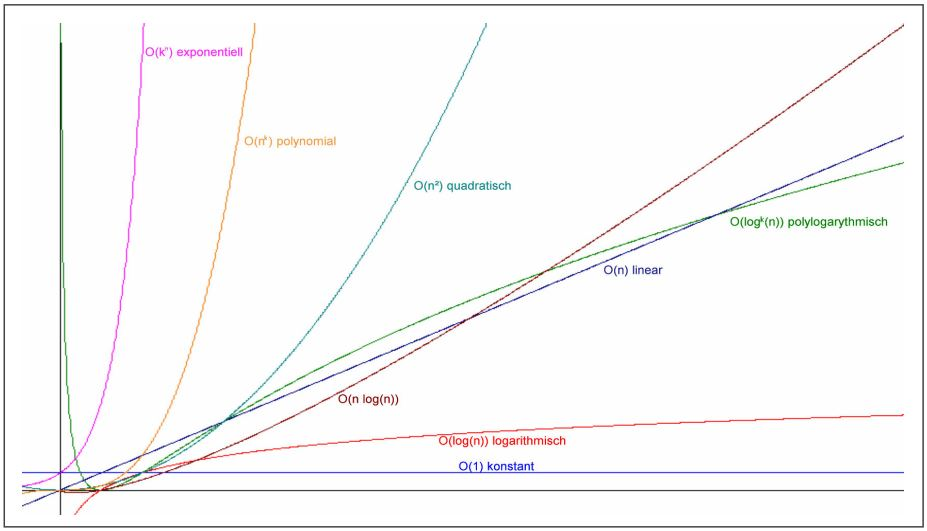
\includegraphics [width=\linewidth]{OWachstum.JPG} \label{fig:WachstumONotation}
\caption{Überblick der einzelnen Funktionen und deren Verlauf \cite{Rehn2006Sortieralgorithmen}}
\end{figure}
Es wird sofort deutlich, dass die lineare und die n log n Funktionen ein deutlich niedrigeres Wachstum besitzen als die quadratische.\\Wenn wir nun einen Blick auf unsere O-Notationen werfen: \\

\begin{table}[h]
\centering
\begin{tabular}{llll}
	\hline
	\textbf{Algorithmus} & \textbf{Best Case} & \textbf{Average Case} & \textbf{Worst Case} \\
	\hline
	BubbleSort & O(n) & O($n^{2}$) & O($n^{2}$) \\
InsertionSort & O(n) & O($n^{2}$) & O($n^{2}$) \\
SelectionSort & O($n^{2}$) & O($n^{2}$) & O($n^{2}$) \\
MergeSort & O(n log n) & O(n log n) & O(n log n) \\
QuickSort & O(n log n) & O(n log n) & O($n^{2}$) \\
HeapSort & O(n log n) & O(n log n) & O(n log n) \\
	\hline
\end{tabular}
\caption{O(Notation) der vorgestellten Algorithmen \cite{India2015Dataset}}
\label{tab:HeapSort}
\end{table}
Nun wäre es aber fahrlässig nur ahand der O-Notation einen Algorithmus auszuwählen. Denn wie im Kapitel zur O-Notation bereits erwähnt, werden Konstanten entfernt.  

\subsubsection{Testfälle}
Um die Algorithmen untereinander zu vergleichen wurden einige Testfälle definiert.\\ 
Die Code Grundlagen zu den Algorithmen wurden von folgenden Seiten entnommen: \cite{bubbleSortCode,selectionSortCode,insertionSortCode,mergeSortCode,quickSortCode,heapSortCode}\\\\

\textbf{Zufalls-Werte:} Den einzelnen Algorithmen wurden die glechen Zufallszahlen übergeben und die Zeit gemessen bis diese die Liste sortiert haben. Es wurden Arrays mit der größe von 100.000 Elementen übergeben:
\begin{table}[h]
\centering
\begin{tabular}{llllll}
\hline
\textbf{BubbleSort} & \textbf{SelectionSort} & \textbf{InsertionSort} & \textbf{QuickSort} & \textbf{MergeSort} & \textbf{HeapSort}  \\
\hline
34793,6 & 14644 & 12765,4 & 15,8 & 46,4 & 31,4 \\
\hline
\end{tabular}
\caption{Ergebnisse von Zufallswerten in Milisekunden(Durchschnittswerte)}
\label{tab:random}
\end{table}
\\An diesem Test erkennt man relativ schnell das die logarithmischen Algorithmen einen riesigen Vorteil gegenüber den quadratischen Algorithmen besitzen, wenn es um zufällig sortierte Listen geht.\\


\textbf{Sortierte:} Es wird eine bereits sortierte Liste den einzelnen Sortieralgorithmen übergeben. Dies ist der Best-Case vom BubbleSort , InsertionSort, QuickSort(mit Pivot Element in der Mitte) und dem MergeSort:\\
\begin{table}[h]
\centering
\begin{tabular}{llllll}
\hline
\textbf{BubbleSort} & \textbf{SelectionSort} & \textbf{InsertionSort} & \textbf{QuickSort} & \textbf{MergeSort} & \textbf{HeapSort}  \\
\hline
$<1$ & 14640,6 & $<1$ & 6,4 & 31,2 & 34 \\
\hline
\end{tabular}
\caption{Ergebnisse von bereits Sortierter Liste in Milisekunden(Durchschnittswerte)}
\label{tab:sorted}
\end{table}
%
\\An diesem Testfalll erkennt man die Stärke von O(n) im vergleich zu logarithmischen Algorithmen.\\

\textbf{Absteigend Sortiert:} Den Algorithmen wird eine absteigend sortierte Liste übergeben. Dies ist der Worst-Case des BubbleSorts, InsertionSort und SelectionSorts:
\begin{table}[h]
\centering
\begin{tabular}{llllll}
\hline
\textbf{BubbleSort} & \textbf{SelectionSort} & \textbf{InsertionSort} & \textbf{QuickSort} & \textbf{MergeSort} & \textbf{HeapSort}  \\
\hline
32427,8 & 15290,6 & 30072,2 & 9,2 & 31,2 & 40,8 \\
\hline
\end{tabular}
\caption{Ergebnisse von abgsteigend sortierter Liste in Milisekunden(Durchschnittswerte)}
\label{tab:inverseSorted}
\end{table}


\textbf{Sortiert, mit kleinstem Element am Ende der Liste:} Es wird eine aufsteigend sortierte Liste, mit der besonderheit, das dass letzte Element das kleinste ist, den Algorithmen übergeben:\\
\begin{table}[h]
\centering
\begin{tabular}{llllll}
\hline
\textbf{BubbleSort} & \textbf{SelectionSort} & \textbf{InsertionSort} & \textbf{QuickSort} & \textbf{MergeSort} & \textbf{HeapSort}  \\
\hline
13956,4 & 14553,6 & $<1$ & $<1$ & 34,4 & 31 \\
\hline
\end{tabular}
\caption{Ergebnisse von sortiert, mit kleinstem Element am Ende der Liste in Milisekunden(Durchschnittswerte)}
\label{tab:inverseSortedplus1}
\end{table}

An diesem Test erkennt man, dass der BubbleSort in jedem Durchgang nur einen Tausch durchführen muss, während der SelectionSort in jedem Durchgang tauschen muss. Dies erklärt warum der BubbleSort schneller ist.\\

\textbf{Testfälle mit den logarithmischen Sortieralgorithmen:} Da die Ergebnisse der logarithmischen Tests relativ klein ausfallen, erhöhen wir die Anzahl der Elemente auf 1.000.000:

\begin{table}[h]
\centering
\begin{tabular}{llll}
\hline
\textbf{Testfall} & \textbf{QuickSort} & \textbf{MergeSort} & \textbf{HeapSort} \\
\hline
 \textbf{Zufall} & 159,2 & 425 & 515,4 \\
\textbf{aufsteigend} & 62,6 & 325 & 390,5 \\
\textbf{absteigend} & 63 & 355,6 & 415,4 \\
\textbf{sortiert, ende klein} & 59,8 & 325 & 387,4 \\
\hline
\end{tabular}
\caption{Testfälle mit 1.000.000 Elemente in Milisekunden(Durchschnittswerte) }
\label{tab:logaTests}
\end{table}

\textbf{Worst-Case QuickSort:} Da der QuickSort in keinen bisherigen Testfällen negativ aufgefallen ist, benötigen wir einen spezial Testfall für den Worst-Case des QuickSorts. Der Worst-Case des QuickSorts tritt ein, wenn das Pivot Element das kleinste, oder größte Element ist. Da unser Pivot Element in den bisherigen Testfällen immer das Element in der Mitte war, ändern wir für diesen Test die Pivotwahl. Wir wählen immer das erste Element in der Liste und als Array übergeben wir eine absteigend sortierte Liste:

\begin{table}[h]
\centering
\begin{tabular}{llll}
\hline
\textbf{BubbleSort} & \textbf{QuickSort} & \textbf{Selection} & \textbf{Insertion} \\
\hline
 465,6 & 218,8 & 137,4 & 259,2 \\
\hline
\end{tabular}
\caption{Testfälle mit 10.000 Elemente in Milisekunden(Durchschnittswerte) }
\label{tab:WC_QS}
\end{table}

Die Ergebnisse zeigen, dass der QuickSort im Worst-Case ungefähr gleichauf mit dem InsertionSort ist. Es ist aber zu beachten, dass der QuickSort nur wenige Vertauschungen durchgeführt hat und das dies der Worst-Case des InsertionSorts ist.


\subsubsection{Vergleich der Ergebnisse}

\textbf{BubbleSort:} Der BubbleSort ist wohl einer der am einfachsten zu verstehenden Algorithmen und er bietet weiterhin auch Stabilität und arbeitet In-Place. Das sind leider auch die einzigen Vorteile dieses Algorithmus. Er benötigt im Vergleich zu anderen  $n^{2}$ Algorithmen in einigen Tests um den Faktor zwei mehr Zeit. Weiterhin tritt der Best-Case zu selten ein um wirklich relevant zu sein. Er dient heute hauptsächlich nur dem Einstieg in Sortieralgorithmen und sollte wirklich nur zu Lernzwecken verwendet werden.\\

\textbf{SelectionSort:} Der SelectionSort besitzt immer eine Laufzeit von O($n^{2}$), was ihn von der O-Notation zum schlechtesten Algorithmus macht. Er liefert aber immer eine konstante Laufzeit und ein großer Vorteil ist, dass die Anzahl der Vertauschungen maximal n sind, da in jedem inneren Schleifen Durchlauf nur ein einziges mal getauscht wird. \\

\textbf{InsertionSort:} Der InsertionSort bietet Stabilität und arbeitet In-Place. Im Vergleich zum BubbleSort ist der InsertionSort in allen Bereichen überlegen.\\

\textbf{MegeSort:} Der MergeSort ist der einzige hier vorgestellte Algorithmus der mit einer Laufzeit von O(n log n) die Stabilität der Eingabe gewährt und sollte, falls man die Stabilität benötigt, gewählt werden.  Ein großes Problem ist aber der zusätzliche Hilfsspeicherbedarf von O(n). Dies bedeutet das für eine Liste von zum Beispiel 2GB noch zusätzlich 2GB benötigt werden.\\

\textbf{HeapSort:} Der HeapSort liefert konstante Ergebnisse, die leicht schlechter sind als beim MergeSort. Er achtet nicht auf die Stabilität, arbeitet dafür aber In-Place mit O(1).\\

\textbf{QuickSort:} Der QuickSort schneidet in useren Testfällen am besten ab. Dies erklärt sich dadurch, das der Worst-Case so gut wie nie auftritt. Das Hauptproblem des QuickSorts ist aber die Wahl des Pivot Element, da links und rechts davon jeweils abgeschnitten wird. Am Worst-Case Testfall haben wir das Pivot als erstes Element der Liste gewählt und eine sortierte Liste übergeben. Dies hat dazu geführt, dass in jedem rekursiven Aufruf nur ein Element von der Liste abgeschnitten wurde. Dies bedeutet das auf dem Stack die Funktion n mal liegt. Bei zu großen Eingaben kann dies zu einem Stackoverflow führen. \\



%Die Ergebnisse zeigen das Sortieralgorithmen, die einen Worst-Case von $n^{2}$ besitzen, einen viel zu großen Zeitaufwand benötigen um ihre Sortierarbeit bei großen Eingaben zu verichten. 



\subsubsection{Relevanz der O-Notation}
Anhand der Testfälle erkennt man, das die O-Notation keine genaue Vergleiche zwischen Sortieralgorithmen zulässt. Das ist aber auch nicht ihr Sinn. Mithilfe der O-Notation ist es relativ einfach Algorithmen in eine Laufzeitspalte einzuordnen, um ein Feedback zu dessen Laufzeit zu bekommen. Danach kann man sich mit der richtigen Laufzeit im Vergleich zu anderen Algorithmen auseinandersetzen.


\section{Schluss}
%\subsection{Fazit}
\subsection{Zusammenfassung und Ausblick}
\subsubsection{Fazit}
Ergebnisse zeigen, dass bei dem SelectionSort keine großen Schwankungen zwischen den Testfällen bei konstanter Listengröße gibt. Nicht besser konnte der BubbleSort abschneiden. Der seltene Auftritt der Best-Cases macht ihn nicht zu einem besseren Algorithmus als der SelectionSort. Im Durchschnitt ist der InsertionSort in jedem Gebieten dem BubbleSort überlegen. Der MergeSort is stabil, doch Schwäche zeigt er in der Speicherverwaltung, denn er benötigt doppelt so viel Speicher zum Sortieren. Der QuickSort liefert die besten Ergebnisse und arbeitet In-Place, doch eine Gefahr in den Worst-Case $n^{2}$ zu geraten. Der HeapSort ist nicht stabil, arbeitet In-Place und hat konstantere Ergebnisse als der MergeSort und sein Worst-Case ist ebenso O(n log n).
\subsubsection{Ausblick}
In der Neuzeit werden Sortieralgorithmen aus den vergangen Jahren verarbeitet, kombiniert oder auch weiterentwickelt. Der LibrarySort ist eine direkte Verbesserung des InsertionSorts. Die durchschnittliche Laufzeit des LibrarySort ist O(n log n), besser als die des InsertionSorts O($n^{2}$ ) \cite{librarySort}.
Eine Kombination des QuickSort und des HeapSort ist der IntroSort \cite{introSort}. Dieses Verfahren benutzt zuerst den QuickSort, wechselt aber dann über auf den HeapSort, um das Worst-Case Szenario des QuickSort zu eliminieren.

\section{Literaturverzeichnis}

%\bibliography{mySA_Bib}
\bibliographystyle{ieeetr}
\bibliography{../BibTex/Sortieralgorithmen.bib}

%\section{Anhang} %Vllt später verwenden


\end{document}